\subsection{Caractéristiques pour la représentation et la notation}

\begin{table}[h]
	\centering
	\begin{tabular}{|c|c|c|} \hline
		Pitchs & Instruments & Codes \\ \hline
		51 & ride & rd \\
		55, 59 & crash & cr \\
		00 & charley-main-ouvert & co \\
		00 & charley-main-fermé & cf \\
		00 & charley-pied-ouvert & po \\
		44 & charley-pied-fermé & pf \\
		36 & grosse-caisse & gc \\
		48, 50 & tom-alto & ta \\
		45, 47 & tom-medium & tm \\
		43, 58 & tom-basse & tb \\
		38, 40 & caisse-claire & cc \\
		37 & cross-stick & cs \\ \hline
	\end{tabular}
	\caption{Pitchs et instruments}
	%	\label{tab:exemple}
\end{table}
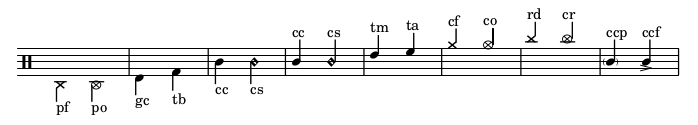
\includegraphics[height=33mm, width=155mm]{z_images/notation/description_notation.png}\\\\
Si la vélocité est en dessous de 40, il s’agit de ghost-notes : la tête de note devra être entouré de parenthèses et le suffixe \textit{p (piano)} devra être ajouté au codes de l’instrument. (Voir ccp ci-dessus.)\\\\
Si la vélocité est au dessus de 90, il s’agit de notes accentuées : le symbole « > » et le suffixe \textit{f (forte)} devra être ajouté au codes de l’instrument. (Voir ccf ci-dessus.)\\\\
Lorsque la vélocité est située entre 40 et 89, on considèrera le volume comme normal et aucun symbole supplémentaire ne sera ajouté à la note.\\\\
L’instrument qui sera difficile à placer sera la caisse claire car elle ne sera pas toujours affiliée aux mêmes instruments.
\subsection{Les systèmes}
Créer un ensemble de systèmes :
\begin{itemize}
\item Trouver les systèmes intéressants dans groove ;
\item Compléter avec des systèmes ago personnalisés ;
\item Tout transcrire avec lilypond et en arbres d’analyse syntaxique.
\item Créer les arbres de voix séparées.
\item Créer les arbres de voix séparées simplifiés (rewriting).\\	
\end{itemize}

\subsubsection{Choix d’écriture}
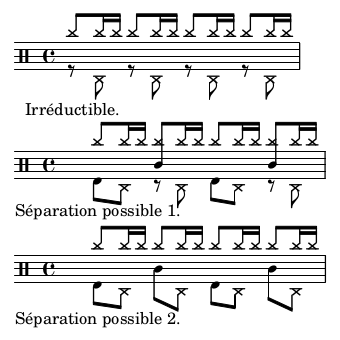
\includegraphics[height=65mm, width=70mm]{z_images/notation/experimentations/separation_drummer_01_session1_004.png}\\
Ici, le système est construit sur un modèle rock en 4/4 : after-beat sur les 2 et 4 avec un choix de répartition des cymbales type fast-jazz.\\
Le système est constitué par défaut du motif ride/ch-pf/cc et d’un texte joué à la grosse-caisse.\\

%\begin{lilypond}[options,go,here]
%	YOUR LILYPOND CODE
%\end{lilypond}

Le motif 1 est privilégié car il réparti selon 2 voix, une voix pour les mains (ride + cc) et une voix pour les pieds (ch-pf + gc). Ce choix paraît plus équilibré car deux instruments sont utilisés par voix et plus logique pour le lecteur puisque les mains sont en haut et les pieds en bas.\\D’autres choix d’écriture auraient été possibles :
\begin{itemize}
	\item Toutes les hampes en haut ;
	\item Combinaison motif 1 et 2 en donnant 2 directions aux hampes de la cc).\\
\end{itemize}
À partir de ce choix d’écriture, le système suivant est défini :\\
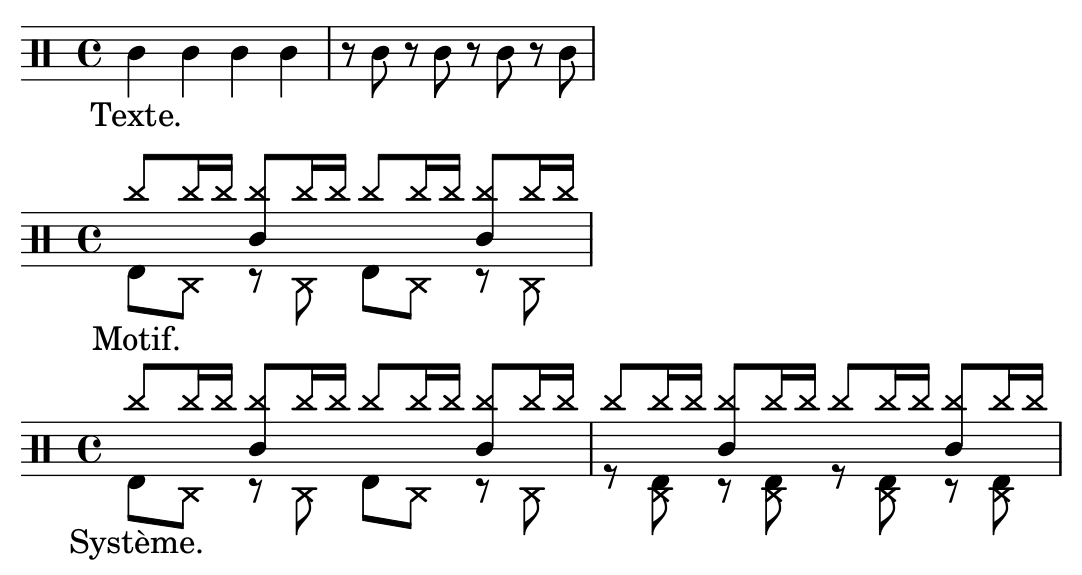
\includegraphics[height=65mm, width=115mm]{z_images/notation/experimentations/system_drummer_01_session1_004.png}\\

Dans le motif, la grosse caisse est notée car elle fait partie de l’équilibre musical de ce rythme mais rigousement, elle ne devrait pas y apparaître puisque qu’elle sera indiquée par le texte.\\
Dans ce système, les noires ne doivent jamais tomber en même temps que les caisse-claires, donc, quand le texte donnera des noires sur les deuxième et quatrième temps, elles ne seront jamais jouées par le batteur (exemple sur la première mesure du système).

\subsubsection{Représentations en arbres}

Quelque soit le choix d’écriture, la représentation arborescente du motif ci-dessus donnera le résultat suivant :

\Tree[ [ [rd\\gc ][ [rd\\pf ][rd ]]]
[ [rd\\cc ][ [rd\\pf ][rd ]]]
[ [rd\\gc ][ [rd\\pf ][rd ]]]
[ [rd\\cc ][ [rd\\pf ][rd ]]] ]\\\\

Représentation du même motif avec les pitchs midi :\\\\
\Tree[ [ [51\\36 ][ [51\\44 ][51 ]]]
[ [51\\38 ][ [51\\44 ][51 ]]]
[ [51\\36 ][ [51\\44 ][51 ]]]
[ [51\\38 ][ [51\\44 ][51 ]]] ]\\\\

Représentation du système (motif + texte) avec les pitchs midi :

\resizebox{420pt}{!}{\Tree[.Système [.Mesure\ 1  [.Temps\ 1 [51\\36 ][ [51\\44 ][51 ]]]
	[.Temps\ 2 [51\\38 ][ [51\\44 ][51 ]]]
	[.Temps\ 3 [51\\36 ][ [51\\44 ][51 ]]]
	[.Temps\ 4 [51\\38 ][ [51\\44 ][51 ]]] ]
	[.Mesure\ 2 [.Temps\ 1 [51 ][ [51\\44\\36 ][51 ]]]
	[.Temps\ 2 [51\\38 ][ [51\\44\\36 ][51 ]]]
	[.Temps\ 3 [51 ][ [51\\44\\36 ][51 ]]]
	[.Temps\ 4 [51\\38 ][ [51\\44\\36 ][51 ]]] ]]}\\

\subsubsection{Séparation des voix}
\resizebox{430pt}{!}{\Tree[.Voix\ haute 
	[.Mesure\ 1 
	[. [rd ][. [rd ][rd ]]]
	[. [rd\\cc ][. [rd ][rd ]]]
	[. [rd ][. [rd ][rd ]]]
	[. [rd\\cc ][. [rd ][rd ]]] ]
	[.Mesure\ 2 
	[. [rd ][. [rd ][rd ]]]
	[. [rd\\cc ][. [rd ][rd ]]]
	[. [rd ][. [rd ][rd ]]]
	[. [rd\\cc ][. [rd ][rd ]]] ]]}\\\\\\
\resizebox{400pt}{!}{\Tree[.Voix\ basse 
	[.Mesure\ 1 
	[. [gc ][. [pf ][tie ]]]
	[. [tie ][. [pf ][tie ]]]
	[. [gc ][. [pf ][tie ]]]
	[. [tie ][. [pf ][tie ]]] ]
	[.Mesure\ 2 
	[. [tie ][. [pf\\gc ][tie ]]]
	[. [tie ][. [pf\\gc ][tie ]]]
	[. [tie ][. [pf\\gc ][tie ]]]
	[. [tie ][. [pf\\gc ][tie ]]] ]]}

\subsubsection{Réécriture (Simplification)}
\resizebox{400pt}{!}{\Tree[.Voix\ basse 
	[.Mesure\ 1 
	[. [gc ][pf ]]
	[. [tie ][pf ]]
	[. [gc ][pf ]]
	[. [tie ][pf ]] ]
	[.Mesure\ 2 
	[. [tie ][pf\\gc ]]
	[. [tie ][pf\\gc ]]
	[. [tie ][pf\\gc ]]
	[. [tie ][pf\\gc ]] ]]}\\\\
La voix haute reste inchangée.
%preamble:
%
%
%%\usetikzlibrary{backgrounds}
%%\usetikzlibrary{trees}
%
%
%Figure 1:
%
%\begin{figure}
%\centering
%\begin{subfigure}
%[$\frac{1}{2} \frac{1}{4} \frac{1}{4}$]
%{
%\begin{tabular}{c}
%%\includegraphics[scale=\scorescale]{images/1a.png}\\
%\begin{tikzpicture} [-,thick]
%\tikzstyle{level 1}=[level distance=7mm,sibling distance=6mm]
%\tikzstyle{level 2}=[level distance=7mm,sibling distance=5mm]
%\node {$\deux$}
%  child { node {$\note$} }
%  child { node {$\deux$}
%    child { node {$\note$} }
%    child { node {$\note$} } };
%\end{tikzpicture}
%\end{tabular}
%%\label{fig:subfig1a}}
%%
%\hspace{0.6cm}
%\begin{subfigure}
%[$\lbrack \frac{1}{6} \rbrack\, \frac{1}{6}\,
%  \lbrack \frac{1}{6} \rbrack\, \frac{1}{6}\,
%  \lbrack \frac{1}{6} \rbrack\, \frac{1}{6}$]
%{
%\begin{tabular}{c}
%%\includegraphics[scale=\scorescale]{images/1b.png}\\
%\begin{tikzpicture} [-,thick]
%\tikzstyle{level 1}=[level distance=7mm,sibling distance=9mm]
%\tikzstyle{level 2}=[level distance=7mm,sibling distance=5mm]
%\node {$\trois$}
%  child { node {$\deux$}
%    child { node {$\rest$} }
%    child { node {$\note$} } }
%  child { node {$\deux$}
%    child { node {$\rest$} }
%    child { node {$\note$} } }
%  child { node {$\deux$}
%    child { node {$\rest$} }
%    child { node {$\note$} } };
%\end{tikzpicture}
%\end{tabular}
%%\label{fig:subfig1b}}
%%
%\hspace{0.6cm}
%\subfig
%[$\frac{1}{5} \frac{1}{5}
%  \frac{1}{15}\frac{1}{15}\frac{1}{15}
%  \frac{1}{5} \frac{1}{5}$]
%{
%\begin{tabular}{c}
%%\includegraphics[scale=\scorescale]{images/1c.png}\\
%\begin{tikzpicture} [-,thick]
%\tikzstyle{level 1}=[level distance=7mm,sibling distance=5mm]
%\tikzstyle{level 2}=[level distance=7mm,sibling distance=5mm]
%\node {$\cinq$}
%  child { node {$\note$} }
%  child { node {$\note$} }
%  child { node {$\trois$}
%    child { node {$\note$} }
%    child { node {$\note$} }
%    child { node {$\note$} } }
%  child { node {$\note$} }
%  child { node {$\note$} } ;
%\end{tikzpicture}
%\end{tabular}
%\label{fig:subfig1c}}
%%
%\begin{RR}
%\hspace{0.6cm}
%\subfig
%[$\frac{1}{12} \frac{1}{12} \frac{1}{12} \frac{1}{12} \frac{1}{3}
%\frac{1}{12} \frac{1}{12} \frac{1}{12} \frac{1}{12}$]
%{
%\begin{tabular}{c}
%%\includegraphics[scale=0\scorescale]{images/1d.png}\\
%%\hspace{0.3cm}
%\begin{tikzpicture} [-,thick]
%\tikzstyle{level 1}=[level distance=7mm,sibling distance=9mm]
%\tikzstyle{level 2}=[level distance=6mm,sibling distance=8mm]
%\tikzstyle{level 3}=[level distance=6mm,sibling distance=5mm]
%\node {$\trois$}
%  child { node {$\deux$}
%    child { node {$\deux$}
%      child { node {$\note$} }
%  child { node {$\note$} } }
%    child { node {$\deux$}
%      child { node {$\note$} }
%  child { node {$\note$} } } }
%  child { node {$\note$} }
%  child { node {$\deux$}
%    child { node {$\deux$}
%      child { node {$\note$} }
%  child { node {$\note$} } }
%    child { node {$\deux$}
%      child { node {$\note$} }
%  child { node {$\note$} } } };
%\end{tikzpicture}
%\end{tabular}
%\label{fig:subfig1d}}
%\end{RR}
%\caption{Simple trees of $\T(\Sigmar)$ with their corresponding
%rhythmic notations and values.}
%\label{fig:trees0}
%\end{figure}